\documentclass{report}

% \usepackage{helvet}
% \renewcommand{\familydefault}{\sfdefault}



\usepackage{fullpage}
\usepackage[parfill]{parskip}
\usepackage{setspace}
\onehalfspacing
\usepackage{minted}
\usepackage{booktabs}
\usepackage{amssymb}
\usepackage{amsmath}
\usepackage{tikz}
\usetikzlibrary{shapes}
\usetikzlibrary{calc}
% \usepackage{standalone}
\usepackage{lipsum}
\usepackage{hyperref}
\usepackage[welsh]{babel}
\usepackage{graphicx}

\newtheorem{definition}{Definition}
\newtheorem{theorem}{Theorem}
\newtheorem{proof}{Proof}

\begin{document}
    \begin{titlepage}
    \begin{center}
        \vspace*{5cm}

        \textbf{Dysgu Peirianyddol}

        \vspace{0.5cm}
        Cyflwyniad i algorithmau dysgu peirianyddol yn R a Python

        \vspace{1.5cm}

        \textbf{Alun Owen}

        \vfill

        B.Sc. Traethawd Blwyddyn 3\\

        \vspace{0.5cm}
        Yr Ysgol Mathemateg Caerdydd

        \vspace{1.5cm}

        
\includegraphics[width=0.15\textwidth]{../img/cflogo.pdf}


    \end{center}
\end{titlepage}
    \Huge{\textbf{Diolchadau}}

\normalsize

\vspace{1.5cm}

Hoffwn ddiolch i Dr Geraint Palmer am yr holl gefnogaeth wrth oruchwylio'r prosiect ac yn ogystal fel tiwtor personol yn ystod y flwyddyn ddiwethaf. 

    \tableofcontents
    \listoffigures

    % The actual content:
    \chapter{Cyflwyniad}\label{cha:introduction}

Mi fyddwn yn ysgrifennu fy mhrosiect trydydd flwyddyn am algorithmau dysgu peirianyddol ag sut i'w defnyddio yn R ac Python. Fydd y prosiect yn cael ei ysgrifennu trwy cyfrwn y Gymraeg. Mi fyddwn yn creu traethawd a gwefan i gyfathrebu gwybodaeth am yr algorithmau. Dwi am ysgrifennu am glystyru $k$-cymedr, atchweliad logistaidd ag dosbarthiad na\"{i}f Bayes.

Bydd y tiwtorialau yn cael ei ddangos drwy'r ieithoedd rhaglennu Python ag R, gan taw nhw yw'r ddwy iaith fwyaf poblogaidd ar gyfer dysgu peirianyddol a gwyddor data yn \^{o}l arolwg Kaggle nol yn 2018 \cite{kagglesurvey}. Mae hefyd ganddynt trwyddedau am ddim, sy'n bwysig ar gyfer hygrychedd. Rheswm arall i ddysgu defnyddio'r ieithoedd rhaglennu yma yw bod nhw'n god agored sy'n wahanol i SQL er enghraifft. Gan ei fod nhw'n god agored poblogaidd, mae'n meddwl fod nhw'n cael ei diweddaru yn aml. Cafodd R ei greu gan ystadegwyr a gan fy mod yn creu tiwtorialau am ddysgu peirianyddol o'r ochr ystadegaeth, mae'n gymhelliad i ddefnyddio R. Ar gyfer dysgu Python, nol yn 2019 roedd Python yr iaith rhaglennu ail fwyaf i gael ``pull requests'' ar Github \cite{canran-github}, a Github oedd y gwesteiwr fwyaf o god ffynhonnell yn y byd. Mae Python ag R yn cael ei ystyried i fod yn hawdd dysgu a deall yn gymhariaeth gydag ieithoedd rhaglennu eraill. Gwelwn yn y tiwtorialau i ddod nad yw gweithredu'r algorithmau yn yr ieithoedd hyn yn gymhleth.

\section{Beth yw Dysgu Peirianyddol}\label{sec:intro_pd}

Yn syml, dysgu peirianyddol yw algorithmau i optimeiddio rhyw feini prawf gan ddefnyddio data. Mae rhain yn cynnwys model wedi'i ddiffinio o rhai paramedrau mesuradwy, a'r darn dysgu fydd i optimeiddio gyda pharch tuag at y paramedrau hyn. Gall y model fod yn un disgrifiadol o'r data, neu un sy'n rhagfynegi rhyw agwedd o'r data. Mae dysgu peirianyddol yn defnyddio ystadegaeth i adeiladu'r modelau mathemategol, ac mae cyfrifiadureg yn edrych mwy i mewn i effeithiolrwydd y proses.\cite{dysgu-peirianyddol2}

Nid yw dysgu peirianyddol yn faes newydd, mae wedi bod o gwmpas ers y 50au pan wnaeth Arthur Samuel o IBM creu rhaglen ar y cyfrifiadur i chwarae'r gem draffts. Yr amser hwn cafodd y term ei bathu. Yna drwy ddatblygiadau technolegol diweddar, mae posibilrwyddau ddysgu peirianyddol bron yn ddiddiwedd. Ers cael ei sefydlu yn y 50au, cymerodd tan 1997 i ddatblygu rhaglen a all guro'r chwaraewr gwyddbwyll orau yn y byd. Nid yn unig yw dysgu peirianyddol yn cael ei ddefnyddio i greu rhaglenni gemau, mae nawr yn cael ei ddefnyddio ym mhob math o raglenni megis llawer o apiau ar eich ff\^{o}n fel ``Google Maps'', ``Uber'' i ``Netflix'' \cite{cymwysiadaudysgupeirianyddol}.

Mae sylfaeni ddysgu peirianyddol yn cael eu defnyddio yn prosesu iaith naturiol a dadansoddi sentiment\cite{technolegau-iaith}. Mae'r proseses yma yn cael ei ddefnyddio i wneud ffwythiannau megis adnabod lleferydd, creu tecst i leferydd a chyfieithiad peirianyddol.
Yn ogystal mae dysgu peirianyddol yn cael ei ddefnyddio i brosesu lluniau, mae'r defnydd yma'n cael ei weld yn aml gyda systemau adnabod wynebau.

Mae dysgu peirianyddol yn cael ei ddefnyddio yn aml i ddadansoddi data pryd bynnag gennym ddata mawr. Mae ein llywodraeth yn defnyddio dysgu peirianyddol yn aml, mae adran actiwari y llywodraeth yn defnyddio dysgu peirianyddol i ddatblygu mewnwelediadau i'w problemau. Hyd yn hyn maen nhw wedi defnyddio dysgu peirianyddol i rannu cynlluniau pensiwn i grwpiau gyda phriodweddau tebyg ac wedi rhagfynegi cyflog graddedigion yn y dyfodol. \cite{GAD}  

Mae deallusrwydd artiffisial wedi tyfu yn esbonyddol yn ddiweddar gyda dysgu peirianyddol. Mae deallusrwydd artiffisial yn y newyddion drwy'r adeg oherwydd datblygiadau parhaus. Yn ddiweddar rydym wedi gweld moduron heb yrrwr, diagnosau meddygol, a `chat bots'.

Categoreiddiwn algorithmau dysgu peirianyddol i ddwy brif fath - dysgu o dan orchwyliaeth, a dysgu heb orchwyliaeth. Maent yn wahanol yn eu pwrpas a'u dulliau.

\subsection{Dysgu dan Oruchwyliaeth}

Diffiniwn $\alpha$ i fod y set o bob label, gall y labeli fod yn arwahanol neu yn ddi-dor, yna diffiniwn $\beta$ fod y fector o ddimensiwn $D \in \mathbb{Z}_{+}$. Gadewch i'n data fod nifer o barau o bwyntiau $(\mathbf{x}_{i},y_{i})$. Yn y fan hyn mae $y_{i} \in \alpha$. Fydd $\mathbf{x}_{i} \in  \beta$ yn fector gyda gwerthoedd ar gyfer priodoleddau gwahanol. Y nod ar gyfer dysgu dan oruchwyliaeth yw dysgu'r mapiad o $\mathbf{x}$ i $y$.\cite{dysgu-peirianyddol}

Gwnawn hyn trwy hollti'r data i mewn i set hyfforddi a set profi, lle mae'n bwysig i dybio pob pwynt wedi'i samplu'n annibynnol a'i dosbarthu o ddosraniad dros $\alpha \times \beta$. Defnyddiwn y set hyfforddi i rhedeg yr algorithm dysgu peiranyddol a chanfod y mapiad. Defnyddiwn y set profi er mwyn gwirio'r mapiad hyn. Fel arfer defnyddiwn tua 70\% o'r data fel y set hyfforddi, a'r 30\% gweddill fel y set profi, er taw tra-baramedr (hyper-parameter) yr hon ac felly gellid ei ddewis.

Mae'r ffurfiau wahanol o ddysgu dan oruchwyliaeth yn cael ei rhannu i ddau faes yn \^{o}l sut fath o ddata sydd gennym. Os yw'r label yn data arwahanol, mae gennym ddosbarthiad (classification). Os yw'r label yn data di-dor, mae gennym atchweliad (regression). Mae yna lwyth o wahanol fathau o ddosbarthiadau ag atchweliadau; dyma ambell o enghreifftiau ohonynt:

\begin{multicols}{2}
\textbf{Dosbarthiad:}

\begin{itemize}
	\item Coed penderfyniadau
	\item Dosbarthiad na\"{i}f Bayes 
	\item $K$ cymydog agosaf
\end{itemize} 

\textbf{Atchweliad:}

\begin{itemize}
	\item Atchweliad logistaidd
	\item Atchweliad llinol
	\item Atchweliad Poisson
\end{itemize}
\end{multicols}

\subsection{Dysgu heb Oruchwyliaeth}

Diffiniwn $\gamma$ i fod yn ddosraniad. Gadewch i'n data fod $X = (x_{1}, \dots, x_{n})$ sy'n dynodi $n$ pwyntiau lle mae $x_{i} \in \gamma$ ag $i \in \{ 1, \dots, n \}$. Tybiwn fod yr enghreifftiau $x_{i}$ wedi'i samplu'n annibynnol a'i dosbarthu o ddosraniad unfath ar $\gamma$. Y nod o ddysgu heb oruchwyliaeth yw amcangyfrif dwysedd o'r dosraniad sy'n debygol o fod wedi creu $X$.\cite{dysgu-peirianyddol}

Mae'r fatha boblogaidd o ddysgu heb oruchwyliaeth yn cymryd ffurf wannach o'r syniad hyn. Dyma ambell i enghraifft ar ffurfiau gwahanol o ddysgu heb oruchwyliaeth:

\begin{itemize}
	\item Clystyru
	\item Lleihad dimensiwn
	\item Model Markov cudd
\end{itemize}

\subsection{Dysgu atgyfnerthol}

Mae dysgu atgyfnerthol yn dysgu drwy wrando ar adborth o'r system ei hyn. Fydd y peiriant yn dysgu i wneud dulliau sy'n arwain tuag at adborth da ac yna yn osgoi unrhyw dullai caiff adborth gwael. Mae hyn yn wahanol i ddysgu dan oruchwyliaeth gan fod does ddim gymaint o ddibyniaeth ar y ddata hyfforddi. Mae'n wahanol i ddysgu heb oruchwyliaeth gan ein bod angen dewis pryd i dderbyn adborth o'r system \cite{technolegau-iaith}. 

Enghraifft o ddysgu atgyfnerthol yw prosesau penderfynu Markov, mae'n cael ei ddiffinio fel proses stocastig dan reolaeth. Mae prosesau penderfynu Markov yn cael ei ddiffinio gan y plyg $(S,A,T,p,r)$. Yn y plyg mae'r newidynnau yn cael ei ddiffinio fel: $S$ yw'r gofod sy'n cynrychioli esblygiad y prosesau, $A$ yw'r set o bob gweithred sy'n bosib, $T$ yw'r set o amseroedd rhwng dewisiadau, $p$ sy'n dynodi'r ffwythiant tebygolrwydd ar gyfer y trosglwyddiad cyflwr ac $r$ sy'n dynodi'r ffwythiant wobrwyo i'r trosglwyddiad cyflwr. Mae prosesau penderfynu Markov yn efelychu system ac yna yn dewis gweithrediadau ar hap ac yn penderfynu ansawdd y dewis drwy'r ffwythiant wobrwyo. Felly fydd y system yn optimeiddio i ddewis yr opsiynau fydd yn allbwn y wobr orau ac felly yn dewis yr opsiwn o'r ansawdd orau.\cite{PPM} 

\section{Adnoddau Cyfrwng Cymraeg ar gyfer Dysgu Peirianyddol}

Dyma'r adnoddau Cymraeg sydd ar gael yn barod yn y faysydd Deallusrwydd Artiffisial, Cyfrifiadureg ag Mathemateg:

\subsection{Gwerthuso adnoddau sy'n bodoli}
\begin{table}[htbt!]

\begin{center}
\rotatebox{90}{%
\begin{tabular}{ | p{0.24\textwidth} | p{0.24\textwidth} | p{0.24\textwidth} | p{0.24\textwidth} | p{0.05\textwidth} | }
\hline
\textit{\textbf{Adnodd}} & \textit{\textbf{Awdur}} & \textit{\textbf{Fformat}} & \textit{\textbf{Cynulleidfa Darged}} & \textit{\textbf{Linc}}\\
\hline
Cwrs `Cyfrifiadureg ar gyfer Mathemateg' yn Python & Dr Vince Knight a Dr Geraint Palmer & Tiwtorial ar wefan & Dechreuwyr mewn codio Python & \cite{Cyfrifiadureg-maths}\\
\hline
Cyrsiau allgyrsiol yn Scratch, HTML, CSS ag Python & Code Club & Tiwtorialau ar y w\^{e} & Plant rhwng $9$ ac $13$ & \cite{codeclub} \\
\hline
Adnoddau ar lawer o testynau wahanol yn cyfrifiadureg & Technocamps & Mewn ffurdd pdf & Plant yn ysgol/coleg & \cite{technocamps} \\
\hline
Cwrs mewn sgiliau ymchwil cyfrifiadurol & Dr Geraint Palmer & Tiwtorialau ar y w\^{e} & Ymchwilwyr & \cite{python-sgiliauymchwil} \\
\hline
Gwybodath ar gydrannau pwysicaf technolegau iaith & Uned technoleg iaith Prifysgol Bangor a Cymen Cyf. & Llawlyfr ar y w\^{e}  & Myfyrwyr, datblygwyr neu academyddion heb gefndir yn y maes & \cite{technolegau-iaith} \\
\hline
ap Botio i hybu rhaglennu i plant & Tinopolis & ap ar cynnyrch apple & Plant rhwng $7$ ac $11$ & \cite{botio} \\
\hline
Enghreifftiau a thiwtorialau o cynnyrch technolegau iaith  &  Uned technoleg iaith Prifysgol Bangor a Cymen Cyf. & Ystorfa ar github & Myfyrwyr, datblygwyr neu academyddion heb gefndir yn y maes & \cite{github-technolegauiaith} \\
\hline
Tiwtorialau Python & Dr Geraint Palmer a Stephanie Jones & Fideos ar Youtube & Dechreuwyr yn rhaglennu gyda Python & \cite{youtube} \\
\hline
Tiwtorialau SQL & pl/sql tiwtorial & Wefan gyda tiwtorialau & Dechreuwyr yn SQL & \cite{sql} \\
\hline
Nodiadau agored am algebra llinol & Dr Alun Morris & Nodiadau (pdf) & Myfyrwyr prifysgol & \cite{Algebra-llinol}\\
\hline
Amrhyw o adnoddau Mathemategol yn dilyn cwricwla CBAC & Dr Gareth Evans & Wefan gyda linciau i wahanol fathau o adnoddau & Myfyrwyr rhwng $11$ a $18$ & \cite{mathemateg} \\
\hline
\end{tabular}%
}
\end{center}\label{fig:tabl}
\caption{Tabl o adnoddau sydd allan yn barod.}
\end{table}


Mae Tabl~\ref{fig:tabl} wedi'i rhannu i adnoddau codio Cymraeg ag i adnoddau mathemategol Cymraeg. Fel gwelwn yn ebrwydd, mae'r nifer o adnoddau codio yn llawer fwy nag rheina o adnoddau mathemategol. Mae'r adnodd \cite{Cyfrifiadureg-maths} yn cychwyn da i unrhyw un sydd gyda diddordeb o gychwyn codio yn Python, mae'n defnydd gwych ar gyfer myfyrwyr mathemateg israddedig gan ei fod yn benodol i fathemateg. Yn ogystal i'r cwrs yma mae gennym hefyd bach o gyflwyniad i Python ar y wefan Sgiliau Ymchwil Ailhynhyrchiadwy \cite{python-sgiliauymchwil}, er bod hyn yn canolbwyntio mwy ar sgiliau fwy eang megis rheolaeth fersiwn a datblygu meddalwedd ymchwil.

\clearpage

Gwelwn yn ogystal fod yna adnoddau ar gyfer rhaglennu yn Python yn Gymraeg ar gael ar YouTube. Ar sianel Geraint Palmer \cite{youtube} mae yna gasgliad o diwtorialau Python. Mae'r tiwtorialau yn cychwyn gyda'r sylfaen o raglennu yn Python ag yn gorffen gyda mynd dros yr algorithm genetig, sy'n mynd law yn llaw gyda fy mhrosiect.
Mae gan y wefan codeclub amrywiaeth eang o adnoddau ar gyfer codio \cite{codeclub}. Mae yna gyrsiau ar HTML, CSS, Python a Scratch. Yn ogystal mae yna brosiectau pellach sy'n gweithredu Raspberry Pi. 

Gwelwn gydag adnodd technocamps \cite{technocamps}, fod yna amrywiaeth eang o adnoddau yn fan hyn fyd. Mae'r wefan wedi'i thargedu i oedran h\^{y}n na'r wefan codeclub. Mae gan technocamps cyrsiau cychwynnol fel y canlynol: CS 101, Deallusrwydd Artiffisial, Greenfoot (Java), Python a Scratch.

Ar wefan technolegau iaith \cite{technolegau-iaith}, mae yna gyflwyniad i'r darnau fwyaf sylfaenol i dechnolegau iaith. Mae yna lawlyfr yn cynnwys gwybodaeth am ddeallusrwydd artiffisial, dysgu dwfn a phrosesu iaith naturiol, mae'n rhoi cyflwyniad i fewn i'r ochr damcaniaethol ohono. Yn rhedeg yn gyfagos i'r wefan yma yw'r ystorfeydd ar GitHub \cite{github-technolegauiaith}. Yn yr ystorfeydd mae yna diwtorial ar sut i greu robot sgwrsio syml drwy ``turing test lessons'', mae'n addas i rhai yng nghyfnod allweddol $2$ a $3$. Mae'n cynnwys tair gwers, un ar sut mae cyfrifiaduron yn meddwl, yr ail ar ydy cyfrifiaduron yn gallu meddwl drostynt eu hynain ag y dwythaf am creu robot sy'n sgwrsio drwy'r defnydd o Raspberry Pi.

Yn y siop ap Apple, fedrem lawrlwytho'r ap botio \cite{botio}. Mae'n ap am chwilota'r gofod am blanedau newydd drwy raglennu. Mae'r ap wedi'i ariannu gan Lywodraeth Cymru ag ar gael am ddim. Cafodd ei greu ar gyfer plant sydd \^{a} diddordeb cael i mewn i raglennu.

Ar yr ochr mathemategol, mae'r adnodd am ddim gan Alun Morris \cite{Algebra-llinol} yn trafod y sylfeini eu hangen i astudio algebra llinol yn mhrifysgol. Mae'r adnodd yma yn enghraifft wych o'r fath o adnoddau mae'r iaith Gymraeg angen fwy ohono. Mae prinder iawn ar adnoddau o'r ansawdd yma yn agored i'r cyhoedd. Mae yna tair prifysgol yn cynnig cyrsiau mathemateg drwy'r Coleg Cymraeg ond dydi dim un yn darparu eu nodiadau drwy borth Coleg Cymraeg. 
Serch hynny mae yna gyfoeth o adnoddau mathemateg Cymraeg ar gyfer addysg o dan $18$ oed, gwelwn hyn gyda'r nifer mawr o adnoddau ar wefan Dr Gareth Evans o Ysgol Creuddyn \cite{mathemateg}.  

Gwelwn fod yna llawer o adnoddau ar gyfer y maes mathemateg a chyfrifiadureg ar gyfer addysg ysgol. Mae yna ddigon o adnoddau i alluogi cenhedlaeth newydd i astudio'r sylfaen gofynnol drwy'r ysgol i astudio unrhyw un o'r ddau yn brifysgol. Unwaith fyddem yn cyrraedd lefel addysg prifysgol, mae'r prinder yn amlwg. Gan fod testunau dysgu peirianyddol yn cynnwys mathemateg o lefel uwch, mae rhaid cael sylfaen datblygedig o destunau mathemateg i'w ddeall. Gallwn ddweud yr un peth am yr angenrheidrwydd o sylfaen datblygedig o gyfrifiadureg. Y broblem sydd gennym yw does yna ddim yr adnoddau yw gwneud gyda mathemateg lefel uwch nag rhaglennu yn R yn y Gymraeg.

\subsection{Yr angen am adnoddau Cyfrwng Cymraeg}

I gychwyn, rwyf eisiau creu gwefan sy'n cynnwys tiwtorialau Cymraeg am algorithmau dysgu peirianyddol oherwydd y prinder ohonyn. Mae yna gymaint o adnoddau ar gyfer pob math o algorithm trwy gyfrwng Saesneg, ond yn Gymraeg, does yna ddim byd o'r fath! Fel gwelwn yn Nhabl~\ref{fig:tabl}, does yna ddim llawer o adnoddau Cymraeg sy'n cynnwys deunydd datblygedig ar gael i'r cyhoedd. O fy mhrofiad personol i, rwyf yn gwybod fod prifysgolion yng Nghymru gydag adnoddau drwy'r cyfrwng Cymraeg ar gael i'w myfyrwyr nhw yn unig. Teimlaf fod hyn yn atal y parhad o addysg ar \^{o}l i fyfyrwyr gorffen eu hastudiaethau ffurfiol oherwydd nad oes adnoddau am ddim ar gael. 

Ers i'r iaith Gymraeg cael ei rhoi ar sylfaen gyfartal i Saesneg yn Gymru yn 1993 a chael gwasanaethau cyhoeddus yn y ddwy iaith, mae wedi bod effaith domino i'r sector preifat. Mae prifysgolion yn gyrff preifat ac felly nid yw'n angenrheidiol iddyn nhw ddilyn \cite{prifysgolion}, ond yn 2011 cafodd y coleg Cymraeg ei sefydlu i ornest a hyn. Mae'r coleg yn hybu prifysgolion Cymru i newid i fod yn ddwyieithog drwy weithio yn bartneriaeth gyda nhw. Hyd at heddiw mae yna fwy o fodiwlau yn cael ei gyfieithu a fwy o fodiwlau yn cael ei chynnig drwy gyfrwng y Gymraeg. Ar gyfer y garfan fydd yn graddio yn 2020 dim ond naw modiwl oedd ar gael drwy'r cyfrwng Cymraeg a rhan fwyaf ohonyn nhw yn y flwyddyn gyntaf.

Rheswm arall i wneud yn Gymraeg yw cefnogi prosiect y llywodraeth a'r wlad i gael miliwn o siaradwyr Cymraeg erbyn 2050 \cite{cymraeg2050}. I gymhorthi'r prosiect yma cafodd cynllun ei rhoi allan yn hybu'r defnydd a chynnyrch o adnoddau technolegol Cymraeg \cite{cymraeg2050tech}. Yn ogystal i greu adnoddau mae'r cynllun yn targedu y datblygiad o ddeallusrwydd artiffisial drwy edrych ar brosesu iaith naturiol yn bennaf. Mae creu'r adnodd yma yn Gymraeg yn bodloni'r ddwy adran o'r cynllun, gobeithio bydd yn hybu fwy i gychwyn creu adnoddau addysg uwch yn y maes yma. Un ateb cyflym i'r prinder fysa os fysa'r prifysgolion yn gadael ei adnoddau allan am ddim ar borth coleg Cymraeg, fel bod rhai prifysgolion yn yr Unol Daleithiau America lle mae yna ystorfa o gyrsiau gydag adnoddau agored ar wefannau fel Coursera \cite{coursera}.

\section{Strwythyr}

Fydd y traethawd yma yn cynnwys tair pennod ar algorithm dysgu peirianyddol. Yn pob pennod fydd yna gefndir ar beth yw'r algorithm a pryd fyddem yn ei ddefnyddio, yn ogystal fydd yna gefndir ar sut mae'r algorithm yn gweithio a beth yw'r fathemateg tu \^{o}l i'r algorithm. Yna fydd yna diwtorial o sut i'w defnyddio yn R ac yna tiwtorial arall yn Python.

Ar gyfer y wefan, mae dudalen cartref lle fydd yno linc i bob tiwtorialau yn y ddau Python ag R. Mae'r wefan yn cynnwys y tiwtorialau ag y wybodaeth angenrheidiol i allu gwneud yr algorithmau yn yr iaith rhaglennu o'ch dewis. Dyma yr wefan: \url{https://dysgupeirianyddol.github.io/}.


    \chapter{Clystyru $k$-cymedr}\label{cha:literature}
\section{Cefndir}
Mae clystyru $k$-cymedr yn ffordd o ddysgu heb oruchwyliaeth, mae'n cymryd data heb ei labelu ac yn eu sortio i mewn i $k$ wahanol glwstwr yn yr obaith i ddarganfod rhyw strwythur doedden ddim yn gwybod yn gynharach.

\begin{figure}
\begin{center}
\begin{minipage}{.4\linewidth}
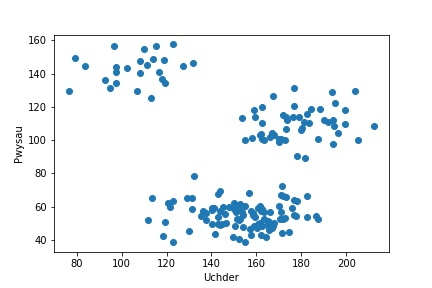
\includegraphics[width=1\linewidth]{../img/Scatterpython.jpeg}
\end{minipage}%
\begin{minipage}{1cm}
$\Rightarrow$
\end{minipage}%
\begin{minipage}{.4\linewidth}
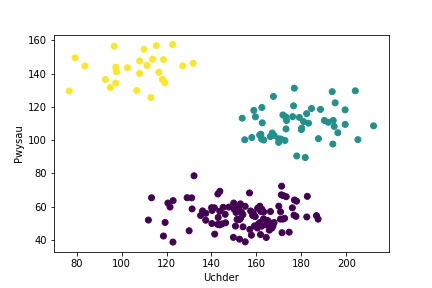
\includegraphics[width=1\linewidth]{../img/3clystwrpython.jpeg}
\end{minipage}%
\label{fig:Cefndir_Clysteru_k_modd}
\caption{Cyn ac ar \^{o}l clystyru $k$-cymedr.}
\end{center}
\end{figure}

I roi enghraifft gwelwch Ddarlun~\ref{fig:Cefndir_Clysteru_k_modd}. Mae'r gwerthoedd ar echelin $x$ yn cynrychioli uchder rhyw berson a'r llall yn cynrychioli pwysau'r person. Fel gwelwn yn y llun ar y chwith gallwn weld tri gr\^{w}p naturiol wedi'i ffurfio. Rydym nawr eisiau eu grwpio yn ffurf Fathemategol. Mae clystyru $k$-cymedr yn medru dosrannu'r tri gr\^{w}p fel gwelwn ar ochr dde'r darlun. 

%%Adio mwy ar sut a pam mae'n cael ei ddefnyddio..

\section{Sut mae Clystyru $K$-cymedr yn gweithio?}

\subsection{Y Dull}

Mae clystyru $k$-cymedr yn syml, mae ond yn dilyn pedwar cam \cite{K-means-clustering}. I wneud yn si\^{w}r fod yn ei ffurf fwyaf cyntefig, fyddan yn defnyddio mesur pellter Ewclidaidd. Yn ogystal mae rhaid dewis $k$ cyn cychwyn y proses. Mae'n bosib optimeiddio'r dewis o $k$, a gwnawn drafod hyn hwyrach ymlaen. Dyma bedwar cam yr algorithm a sut maent yn edrych pan fyddwn ni'n defnyddio'r algorithm ar y data y gwelwn yn \ref{fig:Cefndir_Clysteru_k_modd}:

\begin{enumerate}
\item Aseinio pob elfen i un o'r $k$ clystyrau ar hap.

\begin{figure}[H]
\begin{center}
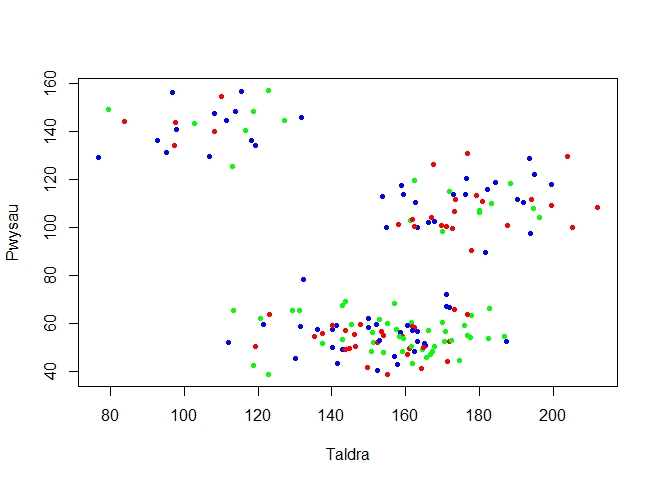
\includegraphics[width=0.5\linewidth]{../img/Cam1.jpeg}
\label{fig:Enghraifft_o_set_cychwynol}
\caption{Enghraifft o set cychwynol ar gyfer clystyru.}
\end{center}
\end{figure}

\item Cyfrifo canolbwynt (hynny yw craidd) pob clwstwr.

\begin{figure}[H]
\begin{center}
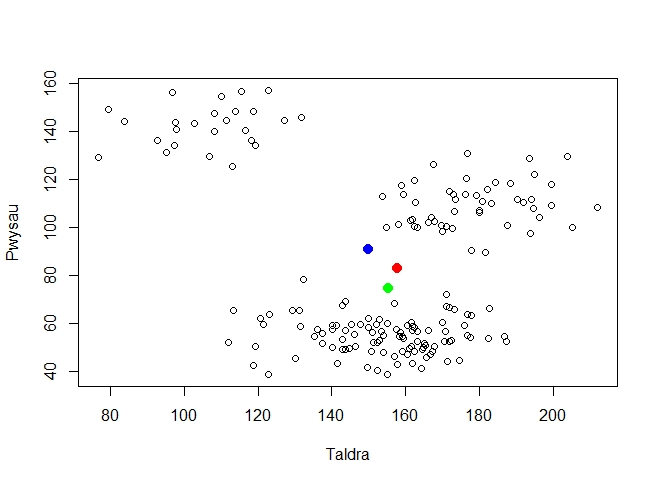
\includegraphics[width=0.5\linewidth]{../img/ClystyrauCychwynol.jpeg}
\end{center}
\end{figure}

\item Ail-aseinio pob elfen unwaith eto i'r clwstwr gyda craidd agosaf.

\begin{figure}[H]
\begin{center}
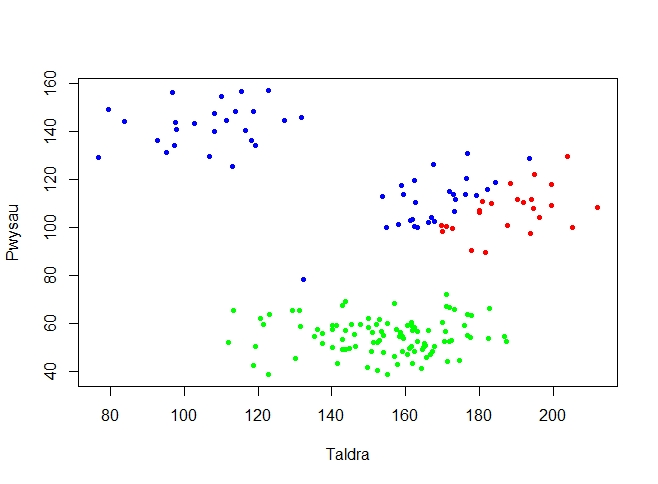
\includegraphics[width=0.5\linewidth]{../img/Cam3.jpeg}
\end{center}
\end{figure}

\item Ailadrodd camau dau a tri tan fod y creiddiau ddim yn symud rhagor.

\begin{figure}[H]
\begin{center}
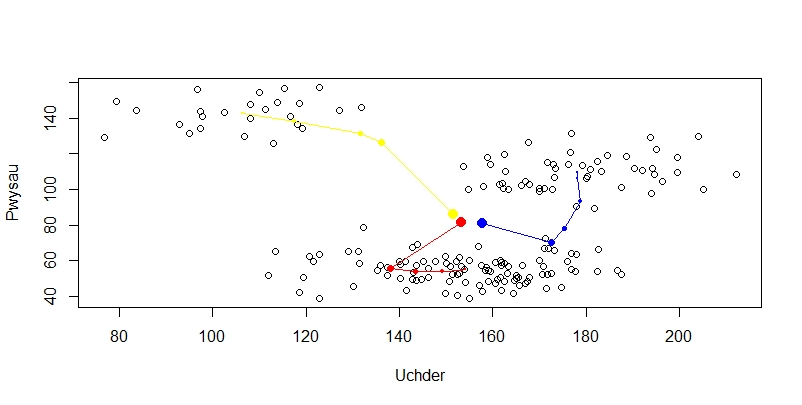
\includegraphics[width=0.5\linewidth]{../img/Convergence4.jpeg}
\end{center}
\end{figure}

\end{enumerate}  

\subsection{Yr Algorithm}

Diffiniwn bob clwstwr rydym yn ceisio darganfod fel $C_i$ lle bydd $i \in \{ 1, 2, \dots, k\}$, mae gennym hefyd $n$ pwyntiau data $x_1, x_2, \dots, x_n$. Gadewch i $\mathbf{c}_i$ bod yn bwynt sy'n graidd i clwstwr $C_i$. Ar gyfer y cam cyntaf angen aseinio pob $\mathbf{x}_j$ i ryw glwstwr $C_i$ ar hap. Yna gan ein bod yn datgelu ein bod yn delio gyda phl\^{a}n Ewclidaidd, mi fyddem yn darganfod craidd pob clwstwr gan y fformiwla ganlynol:

\begin{equation}
\mathbf{c}_i = \frac{1}{|S_i|}\sum_{\mathbf{x}_j \in S_i} {\mathbf{x}_j}
\end{equation}

Yn y fformiwla uchod, gwelwn fod fectorau yn cael eu symio. Fyddem yn gwneud hyn gan symio dros elfennau. \footnote{$ (x_1,x_2,\dots,x_n) + (y_1,y_2,\dots,y_n) = (x_1 + y_1, x_2 + y_2,\dots,x_n + y_n)$}

lle diffiniwn $S_i$ fel y set o bwyntiau data sydd wedi'i aseinio i glwstwr $C_i$.

Nawr mae gan bob clwstwr craidd newydd, fedrwn aseinio pob pwynt data i'r craidd agosaf. Caiff hyn ei gwneud gan fynd drwy bob pwynt data a chyfrifo'r pellter Ewclidaidd \footnote{$|| \mathbf{p} - \mathbf{q} || = \sqrt{(p_1-q_1)^2+(p_2-q_2)^2+\dots+(p_n-q_n)^2}$} i bob canolbwynt. Yna fydd y pwynt priodol yn cael ei labelu gyda'r clwstwr sydd a'r pellter lleiaf o'i graidd i'r pwynt data. Hynny yw

\begin{equation}
\arg \min_{\mathbf{c}_i} ||\mathbf{c}_i, \mathbf{x}_j||^2
\end{equation}

Unwaith mae'r proses wedi'i chychwyn, angen ailadrodd y darn o ddarganfod y creiddiau newydd ac ail labelu'r pwyntiau data tan fod y creiddiau ddim yn symyd rhagor.

\subsection{Sut i ddarganfod y $k$ orau?}

Mae yna wahanol ffurf i ddarganfod $k$, edrychwn ar ddau wahanol ffordd o wneud hyn. 

\subsubsection{Dull Penelin}

Mae'r dull penelin yn cymharu'r cyfanswm o swm sgwariau o fewn y clystyrau. Unwaith gennym y cyfanswm o swm sgwariau o fewn clystyrau i bob $k$ rydym eisiau cymharu, fyddem yn creu plot o bob $k$ yn erbyn y cyfanswm o swm sgwariau o fewn y clystyrau ar gyfer y $k$ hynny. Fydd swm sgwariau ar gyfer clwstwr $C_{i}$ yn cael ei darganfod gan symio y pellter rhwng y craidd $\mathbf{c}_i$ a phob $\mathbf{x}_j$ yn ei tro ag yno ei sgwario fel welwn yn y fformiwla:

$$ SS_{i} = \sum_{j=1}^{n} (\mathbf{x}_{j}-\mathbf{c}_i)^{2} $$

Unwaith mae gennym y graff, allwn ei ddadansoddi. 

\begin{figure}[H]
\begin{center}
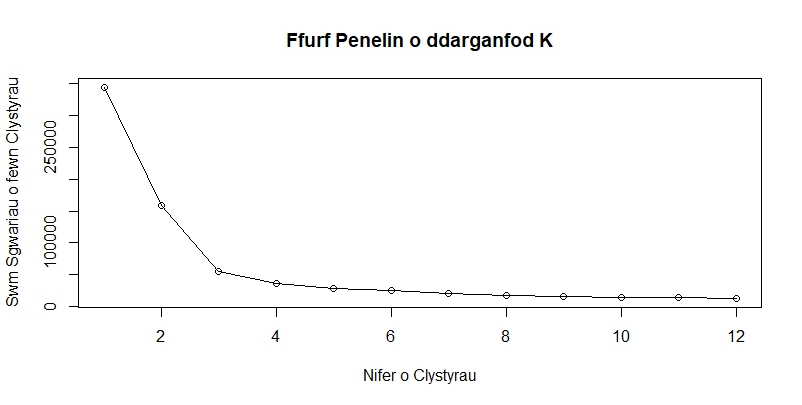
\includegraphics[width=0.5\linewidth]{../img/Dull_Penelin.jpeg}
\caption{Enghraifft o blot o $k$ yn erbyn y cyfanswm swm o sgwariau}
\label{fig:dullpenelin}
\end{center}
\end{figure}

Yn y graff yn Narlun~\ref{fig:dullpenelin}, gwelwn fod swm sgwariau yn fawr yn cychwyn gyda $k$=1 sydd yn gwneud synnwyr. % Pam?
O'r pwynt yma wedyn fydd yna newid mawr yn y swm sgwariau. Unwaith mae'r newid mawr hwn yn dod i ben fydd gennym ongl yn cael ei greu lle bydd newid $k$ dim ond yn creu newid bach. Y pwynt yma fydd yr optimwm ar gyfer nifer $k$ o glystyrau. Fel gwelwn yn glir yn ein henghraifft ni, mae'n glir fod $K$=3 yw dewis orau ar $K$.

\subsubsection{Dendrogram}

Mae dendrogram yn ffordd wahanol iawn i canfod y nifer orau $k$ o glystyrau. Mae'n defnyddio darn o glystyru hierarchaidd i greu diagram canghennog. Mae'r echelin llorweddol yn dangos pob gwrthrych yn ein set o ddata. Mae'r echelin fertigol yn dangos mesur o annhebygrwydd. Mae Darlun~\ref{fig:dendogram} yn dangos dendogram ar gyfer yr un data.

\begin{figure}[H]
\begin{center}
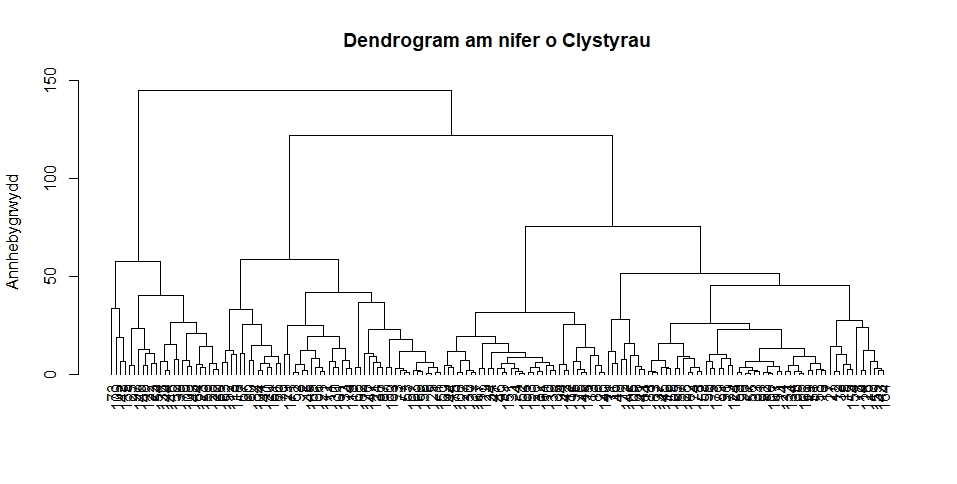
\includegraphics[width=0.5\linewidth]{../img/Dendrogram.jpeg}
\end{center}
\caption{Enghraifft o dendogram}
\label{fig:dendogram}
\end{figure}

I ddadansoddi'r dendrogram mi fyddwn edrych yn bennaf ar yr echelin fertigol. Edrychwn allan am yr annhebygrwydd fwyaf rhwng cyflwyniad o gangen arall yn y goeden. Welwn ni hyn yn ein henghraifft ni ar ôl i'r drydydd clwstwr cael ei gyflwyno yn dendrogram. Mae hyn yn datganu'r un peth a'r dull penelin.

\section{Tiwtorial yn R}
Mi fyddwn yn edrych ar ddata o uchder a phwysau 175 wahanol berson. Mi allwch chi lawrlwytho y data yma o fan hyn. % Cofia ychwanegu'r link

Yno fydd angen lawrlwytho a gosod y pecynnau \mintinline{R}{graphics}, \mintinline{R}{stats} ag \mintinline{R}{datasets} ar eich cyfrifiadur. Ffordd hawdd i wirio hyn fydd i ddefnyddio'r c\^{o}d canlynol: 

\begin{minted}[bgcolor=green!7]{r}
install.packages("graphics")
install.packages("stats")
install.packages("datasets")
library(graphics)
library(stats)
library(datasets)
\end{minted}

Mae'r darn gyntaf o'r c\^{o}d uchod yn gosod/diweddaru'r pecynnau angenrheidiol. Mae'r ail ddarn yn llwytho'r pecynnau i ein sesiwn ni.

Nawr mi wnawn lwytho'r data.

\begin{minted}[bgcolor=green!7]{r}
uchderpwysau <- read.csv("C:/Users/User/Desktop/Dysgu_Peirianyddol/heightvsweight.csv")
View(uchderpwysau)
\end{minted}

Mae'r string sydd mewnbwn y ffwythiant \mintinline{R}{read.csv} yn cyfeirio at y lleoliad ar ein cyfrifiadur lle gallwn ganfod y ffeil csv priodol. Rhaid gwneud yn si\^{w}r eich bod yn defnyddio'r lleoliad cywir i'r lleoliad o'ch ffeil chi.
Ar \^{o}l rhedeg y c\^{o}d ddylai eich data edrych yn debyg i'r canlynol: 

\begin{figure}[H]
\begin{center}
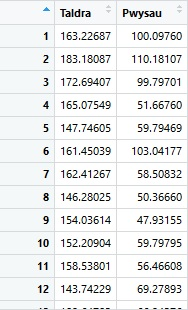
\includegraphics[width=0.35\linewidth]{../img/Data_yn_R.jpg}
\end{center}
\label{fig:DataR}
\end{figure}

Gan fod y data hefo enwau ar gyfer y colofnau, gallwn atodi'r data i lwybr chwilio R. Bydd hyn yn gadael i ni gyfeirio at enwau colofnau'r data yn ein c\^{o}d fydd yn gwneud yn lawer mwy symlach i ddeall.

\begin{minted}[bgcolor=green!7]{r}
attach(uchderpwysau)
\end{minted}

I wneud fwy o synnwyr o'r data, mi wnawn blotio'r data.

\begin{minted}[bgcolor=green!7]{r}
plot(Uchder, Pwysau, pch = 21)
\end{minted}

Sy'n rhoi:

\begin{figure}[H]
\begin{center}
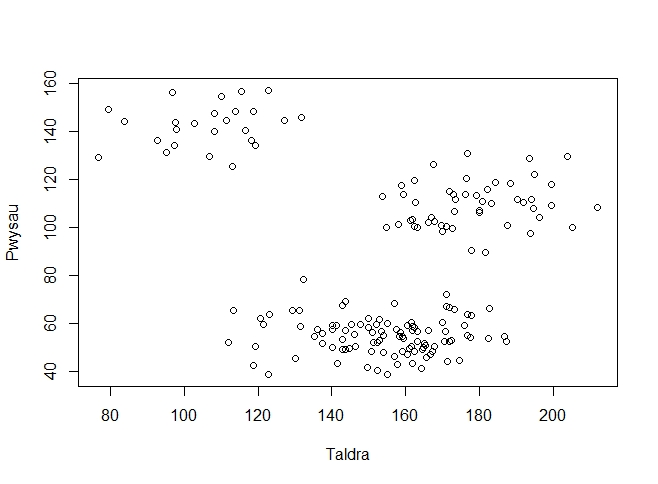
\includegraphics[width=0.5\linewidth]{../img/ScatterplotR.jpeg}
\end{center}
\label{fig:ScatterplotR}
\end{figure}

Gwelwn fod yna 3 clwstwr clir. 

R\^{w}an rydym yn gallu tybio fod y data yn gallu cael i rannu i dri chlwstwr gwahanol, mi wnawn ddefnyddio'r algorithm dysgu peirianyddol i'w ddehongli. Rhedwn y canlynol i redeg clystyru $k$-cymedr yn R. Rydym yn defnyddio'r ymresymiad \mintinline{R}{nstart} i ddewis faint o setiau ar hap o ddata wedi'i labelu wnawn gymered. Welwn enghraifft o'r set ar hap hyn yn Darlun~\ref{fig:Enghraifft_o_set_cychwynol}. Rydym yn neud hyn i wneud yn fwy debygol i ni ddarganfod yr uchafbwynt eang, mae hyn oherwydd mae yna gymaint o uchafbwyntiau lleol.

\begin{minted}[bgcolor=green!7]{r}
kcymedr <- kmeans(uchderpwysau,3, nstart = 50)
\end{minted}

Allwn nawr adio colofn newydd i'r data sef y clystyrau newydd mae'r algorithm wedi'i darganfod.

\begin{minted}[bgcolor=green!7]{r}
uchderpwysau$Clwstwr3 <- kcymedr$cluster
\end{minted}

Gallwn weld y newid hwn gan ddefnyddio'r un c\^{o}d a ddefnyddion yn gynharach.

\begin{minted}[bgcolor=green!7]{r}
View(uchderpwysau)
\end{minted}

\begin{figure}[H]
\begin{center}
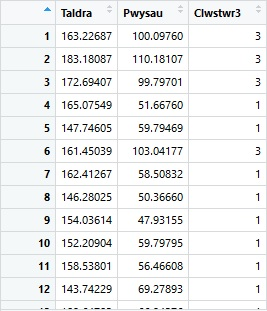
\includegraphics[width=0.5\linewidth]{../img/Data3_yn_R.jpg}
\end{center}
\end{figure}

Mae'n bosib fydd yr algorithm wedi labeli'r clystyrau gwahanol gyda rhifau gwahanol i'r hyn a welwch fan hyn, ddylai'r clystyrau ei hun fod yn hafal. Mae hyn oherwydd y setiau ar hap cychwynnol mae'r algorithm yn ei gymered i gychwyn.

Rhedwn y c\^{o}d canlynol liwio'r clystyrau newydd ar graff.

\begin{minted}[bgcolor=green!7]{r}
plot(Uchder, Pwysau, pch = 21, bg=c("red","green","blue")[unclass(kcymedr$cluster)])
\end{minted}

Sy'n rhoi:

\begin{figure}[H]
\begin{center}
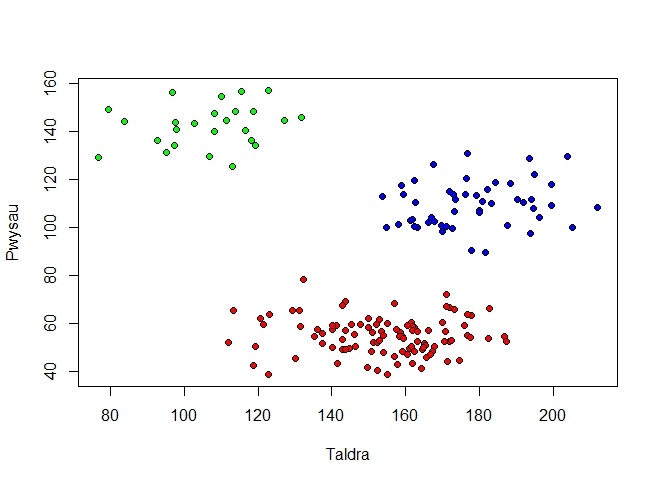
\includegraphics[width=0.5\linewidth]{../img/3clwstwrR.jpeg}
\end{center}
\end{figure}

I gymharu, nawr mi nawn rhedeg yr algorithm ar gyfer 6 clwstwr i weld y clystyrau pan fydd $k=6$. 

\begin{minted}[bgcolor=green!7]{r}
kcymedr <- kmeans(uchderpwysau,6, nstart = 50)
uchderpwysau$Clwstwr6 <- kcymedr$cluster
View(uchderpwysau)
\end{minted}

\begin{figure}[H]
\begin{center}
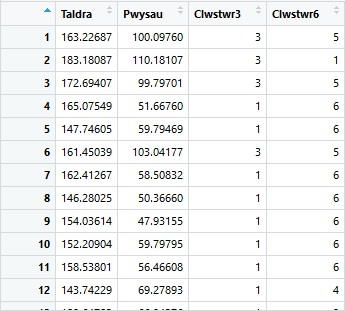
\includegraphics[width=0.5\linewidth]{../img/Data6_yn_R.jpg}
\end{center}
\end{figure}

Gwelwn fod y labeli newydd wedi cael ei ychwanegu i'n tabl. Yna gan blotio graff arall, fedrem weld y 6 clwstwr yn gliriach.

\begin{minted}[bgcolor=green!7]{r}
lliwiau <- c("red","green","blue", "yellow", "black", "white")
plot(Uchder, Pwysau, pch = 21, bg=lliwiau[unclass(kcymedr$cluster)])
\end{minted}

Sy'n rhoi:

\begin{figure}[H]
\begin{center}
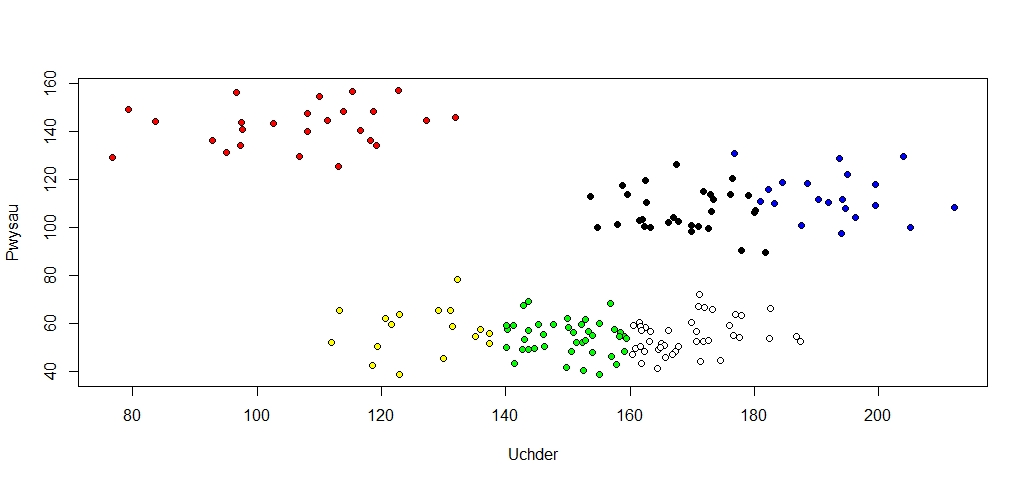
\includegraphics[width=0.5\linewidth]{../img/6clwstwrR.jpeg}
\end{center}
\end{figure}


%Mae'r data iris ar gael iddym drwy'r pecyn "datasets". Yn yr enghraifft top mi wnaethom defnyddio k fel 3, felly hyna be wnawn neud eto.
%Dyma'r c\^{o}d ar gyfer rhedeg clystyru k-cymedr:
%\begin{minted}[bgcolor=green!7]{r}
%clysteru_tri <- kmeans(iris[,1:4],3, nstart = 20)
%clysteru_tri 
%\end{minted}
%Mae'r llinell gyntaf o c\^{o}d yn rhedeg clystyru k-cymedr ar y set data iris gyda k=3. Mae'r darn nstart yn cynrychioli faint o dosraniadau i drio yn cychwyn yn erbyn'r ffwythiant amcan, er mwyn dewis y cychwyn orau. Mae'r ail linell yn allbwn yr wybodaeth canlynol:
%\begin{minted}[bgcolor=green!7]{r}
%>>>K-means clustering with 3 clusters of sizes 50, 62, 38
%>>>
%>>>Cluster means:
%>>>  Sepal.Length Sepal.Width Petal.Length
%>>>1     5.006000    3.428000     1.462000
%>>>2     5.901613    2.748387     4.393548
%>>>3     6.850000    3.073684     5.742105
%>>>  Petal.Width
%>>>1    0.246000
%>>>2    1.433871
%>>>3    2.071053
%>>>
%>>>Clustering vector:
%>>>  [1] 1 1 1 1 1 1 1 1 1 1 1 1 1 1 1 1 1 1 1 1 1 1
%>>> [23] 1 1 1 1 1 1 1 1 1 1 1 1 1 1 1 1 1 1 1 1 1 1
%>>> [45] 1 1 1 1 1 1 2 2 3 2 2 2 2 2 2 2 2 2 2 2 2 2
%>>> [67] 2 2 2 2 2 2 2 2 2 2 2 3 2 2 2 2 2 2 2 2 2 2
%>>> [89] 2 2 2 2 2 2 2 2 2 2 2 2 3 2 3 3 3 3 2 3 3 3
%>>>[111] 3 3 3 2 2 3 3 3 3 2 3 2 3 2 3 3 2 2 3 3 3 3
%>>>[133] 3 2 3 3 3 3 2 3 3 3 2 3 3 3 2 3 3 2
%>>>
%>>>Within cluster sum of squares by cluster:
%>>>[1] 15.15100 39.82097 23.87947
%>>> (between_SS / total_SS =  88.4 %)
%\end{minted}
%Mae'r c\^{o}d uchod rhoi pob wybodaeth a fysa chi eisiau wybod fel allbwn o'r proses.
%I weld y clysterau allwn plotio graff ar gyfer phob cyfuniad o newidynnau. Mae hyn yn alluogi ni i weld yr gwaith dpsbarthu mae'r algorithm wedi'i neud.
%\begin{minted}[bgcolor=green!7]{r}
%plot(iris[,1:4], pch = 24, bg=c("red","green3","blue")[unclass(clysteru_tri$cluster)])
%\end{minted}
%Yn y ffwythiant "plot" uchod, mae'r darn gynta ohono yn cyfeirio tuag at pa data fydd yn cael ei clysteru. Mae'r ail darn yn penodi be fydd pob pwynt data yn cael ei cynrychioli fel pan %mae'r darn dwythaf yn penodi lliw i pob clwstwr.

%Mi wnawn edrych y nawr ar yr set data iris sy'n boblogaidd iawn yn y maes ystadegaeth a gwyddor data. Mae'r data yn cynnwys mesuriadau uchder ag lled petal a setal 150 planhigyn iris. Yn isod gweler lun o allbwn clystyru k-cymedr yn erbyn y clystyrau gwreiddiol o'r data. Gwelwyd fod yr algorithm yn neud yn wych!


\section{Tiwtorial yn python}
Yn y tiwtorial hwn mi wnawn edrych ar yr un data a welom yn y tiwtorial diwethaf.
I gychwyn bydd rhaid llwytho'r pecynnau \mintinline{python}{pandas}, \mintinline{python}{matplotlib.pyplot} ag \mintinline{python}{sklearn.cluster} drwy redeg y c\^{o}d canlynol:

\begin{minted}[bgcolor=cyan!7]{python}
import pandas as pd
import matplotlib.pyplot as plt
import sklearn.cluster
\end{minted}

Y r\^{w}an mi wnawn lwytho'r data i mewn i'n gwaith gan redeg y c\^{o}d:

\begin{minted}[bgcolor=cyan!7]{python}
data = pd.read_csv('heightvsweight.csv')
\end{minted}

Mae'r string sydd mewnbwn y ffwythiant \mintinline{R}{pd.read_csv} yn cyfeirio at y lleoliad ar ein cyfrifiadur lle gallwn ganfod y ffeil csv priodol. Rhaid gwneud yn si\^{w}r eich bod yn defnyddio'r lleoliad cywir i'r lleoliad o'ch ffeil chi.
Unwaith fydd wedi cael ei llwytho, allwn ni gweld yn fras y data gennym ni. 

\begin{minted}[bgcolor=cyan!7]{python}
data.head()
\end{minted}

\begin{figure}[H]
\begin{center}
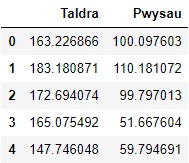
\includegraphics[width=0.35\linewidth]{../img/tabl1.jpg}
\end{center}
\label{fig:Data1}
\end{figure}

I weld y data mewn ffordd fwy gweledol, wnawn blotio graff gwasgariad o'r data.

\begin{minted}[bgcolor=cyan!7]{python}
plt.scatter(data['Uchder'], data['Pwysau']);
plt.xlabel('Uchder')
plt.ylabel('Pwysau')
plt.show()
\end{minted}

\begin{figure}[H]
\begin{center}
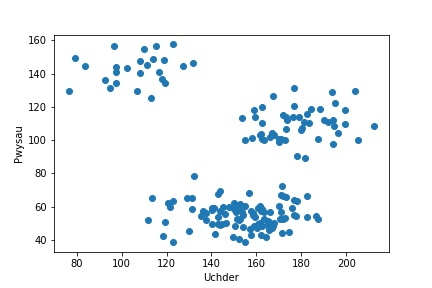
\includegraphics[width=0.7\linewidth]{../img/Scatterpython.jpeg}
\end{center}
\caption{Enghraifft o ddata da i cael ei clystyru.}
\label{fig:Scatterpython}
\end{figure}

Fel gwelwn, mae'r data yn edrych fel ei fod mewn tri chlwstwr. Felly wnawn ddefnyddio'r ffurf algorithm dysgu peirianyddol i'w labelu.

\begin{minted}[bgcolor=cyan!7]{python}
kmeans = sklearn.cluster.KMeans(n_clusters=3).fit(data)
data['Cluster (k=3)'] = kmeans.predict(data)
\end{minted}

Gallwn weld y newid hwn gan ddefnyddio'r un c\^{o}d a ddefnyddion yn gynharach.

\begin{minted}[bgcolor=cyan!7]{python}
data.head()
\end{minted}

\begin{figure}[H]
\begin{center}
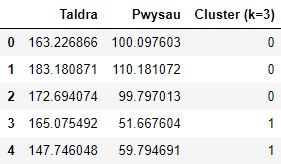
\includegraphics[width=0.35\linewidth]{../img/tabl2.jpg}
\end{center}
\label{fig:Data2}
\end{figure}

Fel y gwelwyd, mae'r data wedi'i rhoi i mewn i dri chlwstwr ac wedi'i labelu gyda rhif y clwstwr. Gan fod pob pwynt yn y data nawr gyda label, allwn ni creu'r plot eto ond gyda bob clwstwr yn lliw gwahanol.

\begin{minted}[bgcolor=cyan!7]{python}
plt.scatter(data['Uchder'], data['Pwysau'], c=data['Cluster (k=3)']);
plt.xlabel('Uchder')
plt.ylabel('Pwysau')
plt.show()
\end{minted}

Sy'n rhoi:

\begin{figure}[H]
\begin{center}
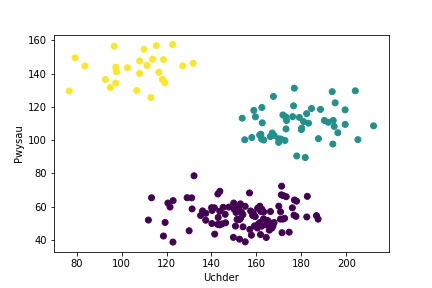
\includegraphics[width=0.7\linewidth]{../img/3clystwrpython.jpeg}
\caption{Sut ddylsa eich graff edrych gyda 3 clystwr.}
\label{fig:3clystwrpython}
\end{center}
\end{figure}

Fel y gwelwn, gweithiodd yr algorithm yn wych. Wnawn nawr trio clystyru $k$-cymedr gyda $k$ yn hafal i 6.

\begin{minted}[bgcolor=cyan!7]{python}
kmeans = sklearn.cluster.KMeans(n_clusters=6).fit(data)
data['Cluster (k=6)'] = kmeans.predict(data)
\end{minted}

Sy'n rhoi:

\begin{minted}[bgcolor=cyan!7]{python}
data.head()
\end{minted}

\begin{figure}[H]
\begin{center}
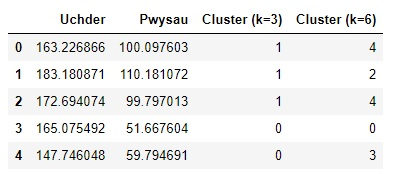
\includegraphics[width=0.35\linewidth]{../img/tabl3.jpg}
\end{center}
\label{fig:Data3}
\end{figure}

Gallwn hefyd gweld canlyniad rhoi'r data i mewn i 6 clwstwr gwahanol: 

\begin{minted}[bgcolor=cyan!7]{python}
plt.scatter(data['Uchder'], data['Pwysau'], c=data['Cluster (k=6)']);
plt.xlabel('Uchder')
plt.ylabel('Pwysau')
plt.show()
\end{minted}

Sy'n rhoi:

\begin{figure}[H]
\begin{center}
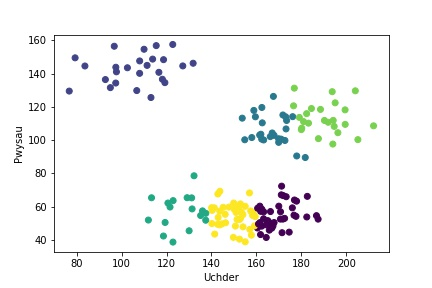
\includegraphics[width=0.7\linewidth]{../img/6clystwrpython.jpeg}
\caption{Sut ddylsa eich graff edrych gyda 6 clystwr.}
\label{fig:6clystwrpython}
\end{center}
\end{figure}

Dyma sut dylaf eich data edrych fel ar \^{o}l a phrosesu drwy glystyru 6-cymedr. 

    \chapter{Termau}\label{cha:appendix}



    % The bibliography:
    \bibliographystyle{plain}
    \bibliography{bibliography}
\end{document}